\section{Optimierungsverfahren}
% TODO: Begriff "Konvergenz" im ersten paragrah erklären, dann in metaheuristiken in Relation stellen zu diversifizierung und intensivierung und in hybride heuristiken als motivation aufgreifen!

% TODO: Einordnung von Evolutionären Algorithmen innerhalb der Metaheuristiken spezifizieren (populationsbasiert und stochastisch) (in zweiter Grafik) ggf Beispiele für andere Kategorien anführen

Im vorherigen Abschnitt haben wir uns unter anderem damit befasst wie die Parameter eines HMMs mittels des Baum-Welch Algorithmus optimiert werden können. In diesem Kapitel treten wir einen Schritt zurück und beantworten die Fragen was es überhaupt bedeutet Dinge zu optimieren und welche verschiedenen Optimierungsansätze existieren.

\subsection*{Was ist Optimierung}
Wir sprechen von einem \textbf{Optimierungsproblem} wenn wir optimale Parameter eines Systems bestimmen wollen. Als Optimale Parameter bezeichnen wir solche, die eine Problemspezifische \textbf{Zielfunktion} $f$ minimieren (oder maximieren). Die Domäne der Zielfunktion nennt man einen \textbf{Suchraum} $S$. Der Wert der Zielfunktion für eine Kombination von Parametern aus dem Suchraum gibt die \textbf{Qualität} dieser Parameter an. Oft gibt es Einschränkungen für die Parameter, so dass nicht alle Werte des Suchraumes mögliche Lösungen sind. Den Raum aller möglichen Lösungen nennen wir \textbf{zulässige Region} \cite*{MetaheuristicsEGT}.

Um diese Konzepte zu verdeutlichen betrachten wir das bekannte Problem des Handlungsreisenden (traveling salesman problem), in welchem es darum geht den Besuch mehrerer Städte optimal zu planen, so dass jede Stadt außer dem Starpunkt nur einmal besucht wird und der Endpunkt equivalent zu dem Startpunkt ist. Der Suchraum ist in diesem Fall gegeben durch alle möglichen Routen (Kombinationen der zu besuchenden Städte). Die Zielfunktion, welche wir minimieren wollen gibt die gesamte Länge einer Reiseroute an. In der zulässigen Region des Suchraumes befinden sich ausschließlich Routen in welchen jede Stadt, bis auf den Startpunkt, einmal besucht wird und der Endpunkt equivalent zum Startpunkt ist. Da Teleportation noch nicht erfunden wurde ist die zulässige Region zusätzlich eingeschränkt auf alle Routen in welchen nacheinander besuchte Städte durch eine Strecke verbunden sind.

\subsection*{Kategorien von Optimierungsverfahren}
Eine Optimierungsmethode, welche stets die global optimale Lösung findet nennt man eine \textbf{exakte Methode}. Für viele Probleme gibt es jedoch keine exakten Algorithmen die eine Lösung in polynomieller Zeit finden. In solch einem Fall kann man zu einer \textbf{Heuristik} greifen. Eine Heuristik liefert eine Lösung die "gut genug" ist in "annehmbarer Zeit". Es handelt sich also um ein Verfahren, welches man umgangssprachlich als Faustregel bezeichnen würde. Eine Heuristik ist nicht das selbe wie ein \textbf{Approximationsalgorithmus}. Denn ein Approximationsalgorithmus garantiert eine untere Schranke für die Qualität einer gefundenen Lösung. Bei einer Heuristik verhält es sich ähnlich wie mit Privatkäufen über Kleinanzeigenportale: Es besteht keine Garantie. Die gefundenen Lösungen eines heuristischen Verfahrens können also beliebig schlecht sein. Heuristiken werden unterteilt in \textbf{spezifische Heuristiken} und \textbf{Metaheuristiken}. Spezifische Heuristiken sind, wie der Name bereits vermuten lässt zugeschnitten auf ein spezifisches Problem, wohingegen Metaheuristiken sehr allgemein sind und auf fast alle Optimierungsprobleme angewendet werden können \cite*{MetaheuristicsEGT}. Metaheuristiken kann man weiter unterteilen in 

Die wahrscheinlich bekannteste Heuristik ist eine \textbf{lokale Suche}. Der Baum-Welch Algorithmus zum Beispiel ist eine lokale Suche. Genetische Algorithmen, mit welchen wir uns später im Detail beschäftigen zählen zu den bekanntesten und ältesten Metaheuristiken.

Figur \ref{fig:optimierungsverfahren} zeigt die zuvor beschriebene Unterteilung der Optimierungsverfahren. Es sei angemerkt, dass die unternommene Unterteilung keineswegs Anspruch auf Vollständigkeit erhebt, sondern primär zur Einordnung des Baum-Welch Algorithmus und des genetischen Algorithmus im Kontext der Optimierungsverfahren dient.
\begin{figure}[h!]
    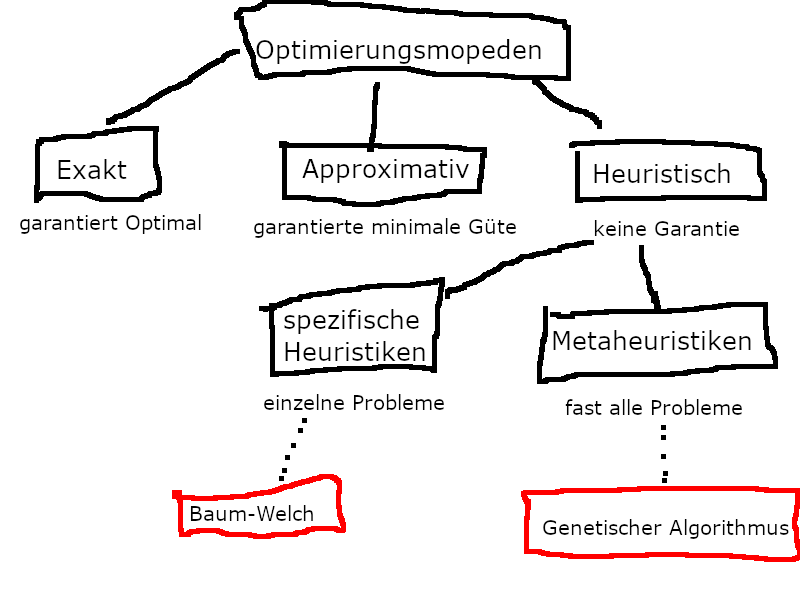
\includegraphics[scale=1.0]{images/Unterteilung_Optimierungsverfahren.png}
    \caption{Unterteilung der Optimierungsverfahren}
    \label{fig:optimierungsverfahren}
\end{figure}

\subsection*{Vergleich von Optimierungsalgorithmen}
Zum Vergleich von Optimierungsalgorithmen ist es wichtig im Hinterkopf zu behalten, dass kein universal guter Optimierungsalgorithmus existieren kann. Das No Free Lunch Theorem postuliert, das für jedes Paar von Algorithmen, unter Betrachtung aller möglichen Optimierungsprobleme, beide Algorithmen im Durchschnitt gleich gut sind \cite*{NFL}. Daraus folgt: wenn Algorithmus $A$ für eine Menge von Problemen besser ist als Algorithmus $B$ muss Algorithmus $B$ für alle restlichen Probleme besser sein als Algorithmus $A$.